\clearpage
\section{Efficiencies and systematic uncertainties for simplified models\label{app:signal}}

\subsection{T2cc\label{app:t2cc}}

\begin{figure}[h!]
  \begin{center}
    \subfigure[Hadronic Selection Efficiency, (2--3,0)]{
      \includegraphics[width=0.4\textwidth,page=6]{figures/sms/t2cc/v1/T2cc_eff}
    } 
    \subfigure[Hadronic Selection Efficiency, (2--3,1)]{
      \includegraphics[width=0.4\textwidth,page=7]{figures/sms/t2cc/v1/T2cc_eff}
    } 
    \subfigure[Hadronic Selection Efficiency, ($\geq 4$,0)]{
      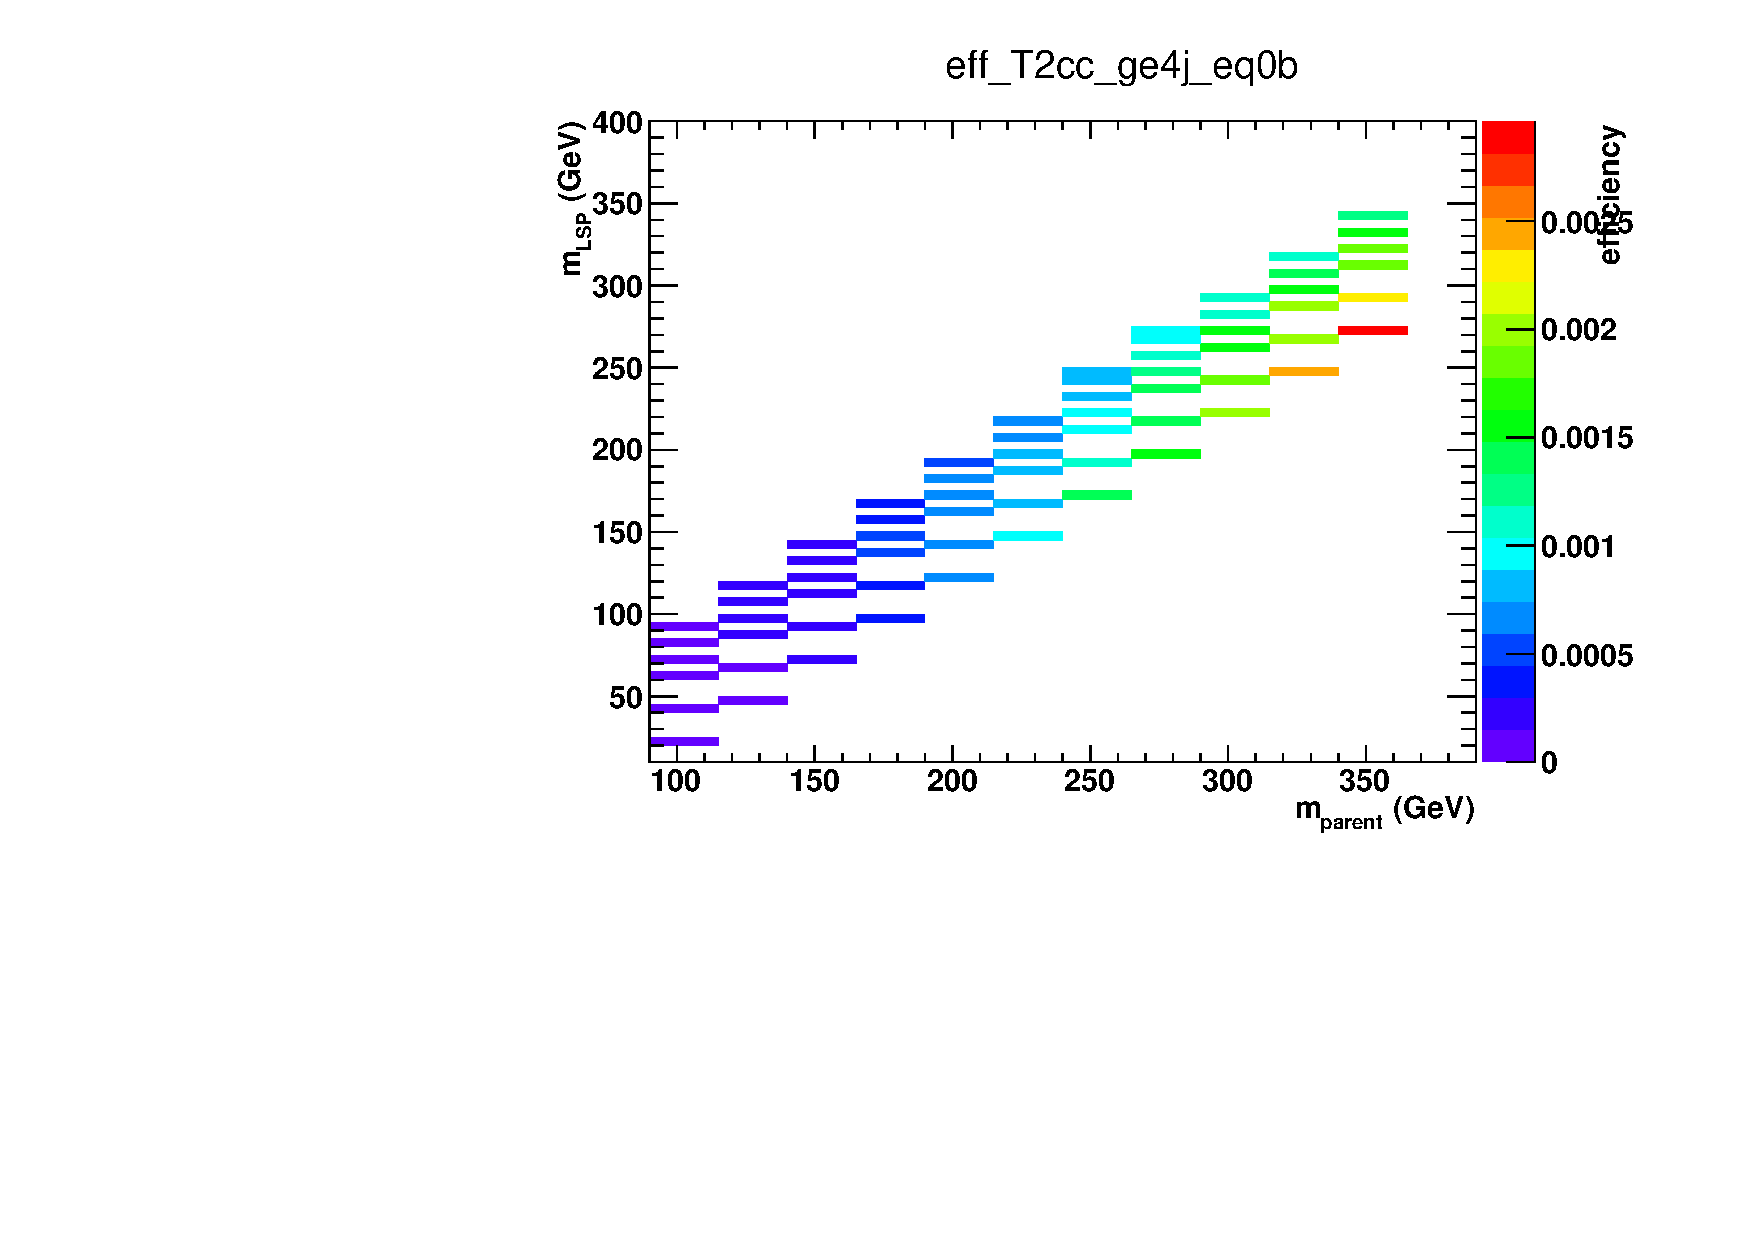
\includegraphics[width=0.4\textwidth,page=1]{figures/sms/t2cc/v1/T2cc_eff}
    } 
    \subfigure[Hadronic Selection Efficiency, ($\geq 4$,1)]{
      \includegraphics[width=0.4\textwidth,page=2]{figures/sms/t2cc/v1/T2cc_eff}
    } 
    \caption{Hadronic selection efficiency times acceptance for \texttt{T2cc}
      for the relevant event categories defined by \njet and \nb.
      Note the different z-axis scales.}
    \label{fig:sms-eff-t2cc}
  \end{center}
\end{figure}

%\begin{figure}[h!]
%  \begin{center}
%    \subfigure[$m_{\sTop} = 250\gev, m_{\rm LSP} = 170\gev$]{
%      \includegraphics[width=0.6\textwidth, trim=0 0 0 30, clip=true]{figures/sms/t2cc/v25/T2cc_sig_inj_250_170}
%    } \\
%%    \subfigure[$m_{\sTop} = 250\gev, m_{\rm LSP} = 230\gev$]{
%%      \includegraphics[width=0.6\textwidth, trim=0 0 0 30, clip=true]{figures/sms/t2cc/v25/T2cc_sig_inj_250_230}
%%    } \\
%    \subfigure[$m_{\sTop} = 250\gev, m_{\rm LSP} = 240\gev$]{
%      \includegraphics[width=0.6\textwidth, trim=0 0 0 30, clip=true]{figures/sms/t2cc/v25/T2cc_sig_inj_250_240}
%    } \\
%    \caption{The expected signal significance (in terms of the number
%      of standard deviations) per signal region bin for the
%      \texttt{T2cc} model with $m_{\sTop} = 250\gev$ and $m_{\rm LSP}
%      = 170\gev$ (Top) and $m_{\rm LSP} = 170\gev$ (Bottom).}
%    % the best fit point $m_{\rm LSP} = 170\gev$ (Middle) 
%    \label{fig:sms-t2cc-sig}
%  \end{center}
%\end{figure}
%
%\begin{figure}[h!]
%  \begin{center}
%    \subfigure[\label{fig:sms-pdf-up-t2cc}$+1\sigma$]{
%      \includegraphics[width=0.6\textwidth]{figures/sms/t2cc/acc_pSigmaRel_m0_m12}
%    }\\
%    \subfigure[\label{fig:sms-pdf-t2cc-nominal}Nominal]{
%      \includegraphics[width=0.6\textwidth]{figures/sms/t2cc/acc_cvRel_m0_m12}
%    }\\
%    \subfigure[\label{fig:sms-pdf-down-t2cc}$-1\sigma$]{
%      \includegraphics[width=0.6\textwidth]{figures/sms/t2cc/acc_mSigmaRel_m0_m12}
%    }\\  
%    \caption{\label{fig:sms-pdf-t2cc}Ratio of efficiency times
%      acceptance for the (middle) central value, (top) $+1\sigma$
%      value, (bottom) $-1\sigma$ value of the envelope calculation
%      relative to the nominal PDF set used to produce the
%      \texttt{T2cc} sample. }
%  \end{center}
%\end{figure}
%
%\begin{figure}[h!]
%  \begin{center}
%    \subfigure[\njetlow, $\nb = 0$.]{
%      \includegraphics[width=0.35\textwidth, page=4]{figures/sms/t2cc/v25/T2cc_JES_eq0b_le3j}
%    }
%    \subfigure[\njetlow, $\nb = 0$.]{
%      \includegraphics[width=0.35\textwidth, page=6]{figures/sms/t2cc/v25/T2cc_JES_eq0b_le3j}
%    }
%    \subfigure[\njetlow, $\nb = 0$.]{
%      \includegraphics[width=0.35\textwidth, page=7]{figures/sms/t2cc/v25/T2cc_JES_eq0b_le3j}
%    }\\
%    \subfigure[\njetlow, $\nb = 1$.]{
%      \includegraphics[width=0.35\textwidth, page=4]{figures/sms/t2cc/v25/T2cc_JES_eq1b_le3j}
%    }
%    \subfigure[\njetlow, $\nb = 1$.]{
%      \includegraphics[width=0.35\textwidth, page=6]{figures/sms/t2cc/v25/T2cc_JES_eq1b_le3j}
%    }
%    \subfigure[\njetlow, $\nb = 1$.]{
%      \includegraphics[width=0.35\textwidth, page=7]{figures/sms/t2cc/v25/T2cc_JES_eq1b_le3j}
%    }\\
%    \subfigure[\njethigh, $\nb = 0$.]{
%      \includegraphics[width=0.35\textwidth, page=4]{figures/sms/t2cc/v25/T2cc_JES_eq0b_ge4j}
%    }
%    \subfigure[\njethigh, $\nb = 0$.]{
%      \includegraphics[width=0.35\textwidth, page=6]{figures/sms/t2cc/v25/T2cc_JES_eq0b_ge4j}
%    }
%    \subfigure[\njethigh, $\nb = 0$.]{
%      \includegraphics[width=0.35\textwidth, page=7]{figures/sms/t2cc/v25/T2cc_JES_eq0b_ge4j}
%    }\\
%    \subfigure[\njethigh, $\nb = 1$.]{
%      \includegraphics[width=0.35\textwidth, page=4]{figures/sms/t2cc/v25/T2cc_JES_eq1b_ge4j}
%    }  
%    \subfigure[\njethigh, $\nb = 1$.]{
%      \includegraphics[width=0.35\textwidth, page=6]{figures/sms/t2cc/v25/T2cc_JES_eq1b_ge4j}
%    }
%    \subfigure[\njethigh, $\nb = 1$.]{
%      \includegraphics[width=0.35\textwidth, page=7]{figures/sms/t2cc/v25/T2cc_JES_eq1b_ge4j}
%    }\\
%    \caption{\label{fig:sms-jes-t2cc}The fractional change in
%      signal efficiency due to systematically (Left) increasing and
%      (Middle) decreasing all jet energies, and (Right) the resulting
%      (symmetric) systematic uncertainties due to JES uncertainties
%      for \texttt{T2cc}.}
%  \end{center}
%\end{figure}
%
%\begin{figure}[h!]
%  \begin{center}
%    \subfigure[\njetlow, $\nb = 0$.]{
%      \includegraphics[width=0.35\textwidth, page=4]{figures/sms/t2cc/v25/T2cc_ISR_eq0b_le3j}
%    }
%    \subfigure[\njetlow, $\nb = 0$.]{
%      \includegraphics[width=0.35\textwidth, page=6]{figures/sms/t2cc/v25/T2cc_ISR_eq0b_le3j}
%    }
%    \subfigure[\njetlow, $\nb = 0$.]{
%      \includegraphics[width=0.35\textwidth, page=7]{figures/sms/t2cc/v25/T2cc_ISR_eq0b_le3j}
%    }\\
%    \subfigure[\njetlow, $\nb = 1$.]{
%      \includegraphics[width=0.35\textwidth, page=4]{figures/sms/t2cc/v25/T2cc_ISR_eq1b_le3j}
%    }
%    \subfigure[\njetlow, $\nb = 1$.]{
%      \includegraphics[width=0.35\textwidth, page=6]{figures/sms/t2cc/v25/T2cc_ISR_eq1b_le3j}
%    }
%    \subfigure[\njetlow, $\nb = 1$.]{
%      \includegraphics[width=0.35\textwidth, page=7]{figures/sms/t2cc/v25/T2cc_ISR_eq1b_le3j}
%    }\\
%    \subfigure[\njethigh, $\nb = 0$.]{
%      \includegraphics[width=0.35\textwidth, page=4]{figures/sms/t2cc/v25/T2cc_ISR_eq0b_ge4j}
%    }
%    \subfigure[\njethigh, $\nb = 0$.]{
%      \includegraphics[width=0.35\textwidth, page=6]{figures/sms/t2cc/v25/T2cc_ISR_eq0b_ge4j}
%    }
%    \subfigure[\njethigh, $\nb = 0$.]{
%      \includegraphics[width=0.35\textwidth, page=7]{figures/sms/t2cc/v25/T2cc_ISR_eq0b_ge4j}
%    }\\
%    \subfigure[\njethigh, $\nb = 1$.]{
%      \includegraphics[width=0.35\textwidth, page=4]{figures/sms/t2cc/v25/T2cc_ISR_eq1b_ge4j}
%    }  
%    \subfigure[\njethigh, $\nb = 1$.]{
%      \includegraphics[width=0.35\textwidth, page=6]{figures/sms/t2cc/v25/T2cc_ISR_eq1b_ge4j}
%    }
%    \subfigure[\njethigh, $\nb = 1$.]{
%      \includegraphics[width=0.35\textwidth, page=7]{figures/sms/t2cc/v25/T2cc_ISR_eq1b_ge4j}
%    }\\
%    \caption{\label{fig:sms-isr-t2cc}The fractional change in signal
%      efficiency due to systematically (Left) increasing and (Middle)
%      decreasing event weights according to ISR uncertainties, and
%      (Right) the resulting (symmetric) systematic uncertainties due
%      to ISR uncertainties for \texttt{T2cc}.}
%  \end{center}
%\end{figure}
%
%\begin{figure}[h!]
%  \begin{center}
%    \subfigure[\njetlow, $\nb = 0$.]{
%      \includegraphics[width=0.35\textwidth, page=4]{figures/sms/t2cc/v25/T2cc_bTag_eq0b_le3j}
%    }
%    \subfigure[\njetlow, $\nb = 0$.]{
%      \includegraphics[width=0.35\textwidth, page=6]{figures/sms/t2cc/v25/T2cc_bTag_eq0b_le3j}
%    }
%    \subfigure[\njetlow, $\nb = 0$.]{
%      \includegraphics[width=0.35\textwidth, page=7]{figures/sms/t2cc/v25/T2cc_bTag_eq0b_le3j}
%    }\\
%    \subfigure[\njetlow, $\nb = 1$.]{
%      \includegraphics[width=0.35\textwidth, page=4]{figures/sms/t2cc/v25/T2cc_bTag_eq1b_le3j}
%    }
%    \subfigure[\njetlow, $\nb = 1$.]{
%      \includegraphics[width=0.35\textwidth, page=6]{figures/sms/t2cc/v25/T2cc_bTag_eq1b_le3j}
%    }
%    \subfigure[\njetlow, $\nb = 1$.]{
%      \includegraphics[width=0.35\textwidth, page=7]{figures/sms/t2cc/v25/T2cc_bTag_eq1b_le3j}
%    }\\
%    \subfigure[\njethigh, $\nb = 0$.]{
%      \includegraphics[width=0.35\textwidth, page=4]{figures/sms/t2cc/v25/T2cc_bTag_eq0b_ge4j}
%    }
%    \subfigure[\njethigh, $\nb = 0$.]{
%      \includegraphics[width=0.35\textwidth, page=6]{figures/sms/t2cc/v25/T2cc_bTag_eq0b_ge4j}
%    }
%    \subfigure[\njethigh, $\nb = 0$.]{
%      \includegraphics[width=0.35\textwidth, page=7]{figures/sms/t2cc/v25/T2cc_bTag_eq0b_ge4j}
%    }\\
%    \subfigure[\njethigh, $\nb = 1$.]{
%      \includegraphics[width=0.35\textwidth, page=4]{figures/sms/t2cc/v25/T2cc_bTag_eq1b_ge4j}
%    }  
%    \subfigure[\njethigh, $\nb = 1$.]{
%      \includegraphics[width=0.35\textwidth, page=6]{figures/sms/t2cc/v25/T2cc_bTag_eq1b_ge4j}
%    }
%    \subfigure[\njethigh, $\nb = 1$.]{
%      \includegraphics[width=0.35\textwidth, page=7]{figures/sms/t2cc/v25/T2cc_bTag_eq1b_ge4j}
%    }\\
%    \caption{\label{fig:sms-btag-t2cc}The fractional change in signal
%      efficiency due to systematically (Left) increasing and (Middle)
%      decreasing all b-tag efficiencies according to the scale factor
%      uncertainties, and (Right) the resulting (symmetric) systematic
%      uncertainties due to b-tag scale factor uncertainties for
%      \texttt{T2cc}.} 
%  \end{center}
%\end{figure}
%
%\begin{figure}[h!]
% \begin{center}
%   \subfigure[\njetlow, $\nb = 0$.]{
%     \includegraphics[width=0.35\textwidth, page=4]{figures/sms/t2cc/v25/T2cc_MHT_MET_eq0b_le3j}
%   } \\
%   \subfigure[\njetlow, $\nb = 1$.]{
%     \includegraphics[width=0.35\textwidth, page=4]{figures/sms/t2cc/v25/T2cc_MHT_MET_eq1b_le3j}
%   } \\
%   \subfigure[\njethigh, $\nb = 0$.]{
%     \includegraphics[width=0.35\textwidth, page=4]{figures/sms/t2cc/v25/T2cc_MHT_MET_eq0b_ge4j}
%   } \\
%   \subfigure[\njethigh, $\nb = 1$.]{
%     \includegraphics[width=0.35\textwidth, page=4]{figures/sms/t2cc/v25/T2cc_MHT_MET_eq1b_ge4j}
%   } \\
%   \caption{\label{fig:sms-mht-met-t2cc}The efficiency of the
%     $\mht/\met < 1.25$ requirement, for relative event categories. }
% \end{center}
%\end{figure}
%
%\begin{figure}[h!]
% \begin{center}
%   \subfigure[\njetlow, $\nb = 0$.]{
%     \includegraphics[width=0.35\textwidth, page=4]{figures/sms/t2cc/v25/T2cc_DeadECAL_eq0b_le3j}
%   } \\
%   \subfigure[\njetlow, $\nb = 1$.]{
%     \includegraphics[width=0.35\textwidth, page=4]{figures/sms/t2cc/v25/T2cc_DeadECAL_eq1b_le3j}
%   } \\
%   \subfigure[\njethigh, $\nb = 0$.]{
%     \includegraphics[width=0.35\textwidth, page=4]{figures/sms/t2cc/v25/T2cc_DeadECAL_eq0b_ge4j}
%   } \\
%   \subfigure[\njethigh, $\nb = 1$.]{
%     \includegraphics[width=0.35\textwidth, page=4]{figures/sms/t2cc/v25/T2cc_DeadECAL_eq1b_ge4j}
%   } \\
%   \caption{\label{fig:sms-dead-ecal-t2cc}The efficiency of the dead
%     ECAL filter, for relative event categories. }
% \end{center}
%\end{figure}
%
\begin{figure}[h!]
  \begin{center}
    \subfigure[\njetlow, $\nb = 0$.]{
     \includegraphics[width=0.48\textwidth,page=1]{figures/sms/t2cc/v1/t2cc_pfJet_totalUnc.pdf}
    }                                                                  
    \subfigure[\njetlow, $\nb = 1$.]{                                  
     \includegraphics[width=0.48\textwidth,page=2]{figures/sms/t2cc/v1/t2cc_pfJet_totalUnc.pdf}
    }\\                                                                
    \subfigure[\njethigh, $\nb = 0$.]{                                 
      \includegraphics[width=0.48\textwidth,page=5]{figures/sms/t2cc/v1/t2cc_pfJet_totalUnc.pdf}
    }                                                                  
    \subfigure[\njethigh, $\nb = 1$.]{                                 
      \includegraphics[width=0.48\textwidth,page=6]{figures/sms/t2cc/v1/t2cc_pfJet_totalUnc.pdf}
    }\\
    \caption{\label{fig:sms-total-t2cc}The total systematic
      uncertainty in the signal efficiency times acceptance for all
      relevant event categories for the \texttt{T2cc} intepretation.}
  \end{center}
\end{figure}

%%%%%%%%%%%%%%%%%%%%%%%%%%%%%%%%%%%%%%%%%%%%%%%%%%%%%%%%%%%%%%%%%%%%%%%%%%%%%%%%
%%%%%%%%%%%%%%%%%%%%%%%%%%%%%%%%%%%%%%%%%%%%%%%%%%%%%%%%%%%%%%%%%%%%%%%%%%%%%%%%
%%%%%%%%%%%%%%%%%%%%%%%%%%%%%%%%%%%%%%%%%%%%%%%%%%%%%%%%%%%%%%%%%%%%%%%%%%%%%%%%

%\clearpage
\subsection{T2tt\label{app:t2tt}}

\begin{figure}[h!]
  \begin{center}
    \subfigure[\njetlow, $\nb = 1$.]{
     \includegraphics[width=0.48\textwidth,page=2]{figures/sms/t2tt/v1/t2tt_pfJet_totalUnc.pdf}
    }
    \subfigure[\njetlow, $\nb = 2$.]{
     \includegraphics[width=0.48\textwidth,page=3]{figures/sms/t2tt/v1/t2tt_pfJet_totalUnc.pdf}
    }\\       
    \caption{\label{fig:sms-total-t2tt}The total systematic
      uncertainty in the signal efficiency times acceptance for all
      relevant event categories for the \texttt{T2tt} intepretation.}
  \end{center}
\end{figure}

%%%%%%%%%%%%%%%%%%%%%%%%%%%%%%%%%%%%%%%%%%%%%%%%%%%%%%%%%%%%%%%%%%%%%%%%%%%%%%%%
%%%%%%%%%%%%%%%%%%%%%%%%%%%%%%%%%%%%%%%%%%%%%%%%%%%%%%%%%%%%%%%%%%%%%%%%%%%%%%%%
%%%%%%%%%%%%%%%%%%%%%%%%%%%%%%%%%%%%%%%%%%%%%%%%%%%%%%%%%%%%%%%%%%%%%%%%%%%%%%%%

\clearpage
\subsection{T2tt\label{app:t2tt}}

\begin{figure}[!h]
  \begin{center}
    \subfigure[Hadronic Selection Efficiency, (2--3,1)]{
      \includegraphics[width=0.4\textwidth,page=7]{figures/sms/t2tt/v1/T2tt_eff}
    } 
    \subfigure[Hadronic Selection Efficiency, (2--3,2)]{
      \includegraphics[width=0.4\textwidth,page=8]{figures/sms/t2tt/v1/T2tt_eff}
    } \\
%    \subfigure[Hadronic Selection Efficiency, ($\geq 4$,0)]{
%      \includegraphics[width=0.4\textwidth]{figures/sms/t2_4body/v6/T2_4body_had_eff_maps_eq0b_ge4j_SITV}
%    }     
%    \subfigure[Hadronic Selection Efficiency, ($\geq 4$,1)]{
%      \includegraphics[width=0.4\textwidth]{figures/sms/t2_4body/v6/T2_4body_had_eff_maps_eq1b_ge4j_SITV}
%    } \\
    \caption{Hadronic selection efficiency times acceptance for the \texttt{T2tt}
      for the relevant event categories defined by \njet and \nb.
       Note the different z-axis scales.}
    \label{fig:sms-eff-t2_4body}
  \end{center}
\end{figure}

%\begin{figure}[h!]
%  \begin{center}
%    \subfigure[\njetlow, $\nb = 0$.]{
%      \includegraphics[width=0.35\textwidth, page=4]{figures/sms/t2_4body/v6/T2_4body_JES_eq0b_le3j}
%    }
%    \subfigure[\njetlow, $\nb = 0$.]{
%      \includegraphics[width=0.35\textwidth, page=6]{figures/sms/t2_4body/v6/T2_4body_JES_eq0b_le3j}
%    }
%    \subfigure[\njetlow, $\nb = 0$.]{
%      \includegraphics[width=0.35\textwidth, page=7]{figures/sms/t2_4body/v6/T2_4body_JES_eq0b_le3j}
%    }\\
%    \subfigure[\njetlow, $\nb = 1$.]{
%      \includegraphics[width=0.35\textwidth, page=4]{figures/sms/t2_4body/v6/T2_4body_JES_eq1b_le3j}
%    }
%    \subfigure[\njetlow, $\nb = 1$.]{
%      \includegraphics[width=0.35\textwidth, page=6]{figures/sms/t2_4body/v6/T2_4body_JES_eq1b_le3j}
%    }
%    \subfigure[\njetlow, $\nb = 1$.]{
%      \includegraphics[width=0.35\textwidth, page=7]{figures/sms/t2_4body/v6/T2_4body_JES_eq1b_le3j}
%    }\\
%    \subfigure[\njethigh, $\nb = 0$.]{
%      \includegraphics[width=0.35\textwidth, page=4]{figures/sms/t2_4body/v6/T2_4body_JES_eq0b_ge4j}
%    }
%    \subfigure[\njethigh, $\nb = 0$.]{
%      \includegraphics[width=0.35\textwidth, page=6]{figures/sms/t2_4body/v6/T2_4body_JES_eq0b_ge4j}
%    }
%    \subfigure[\njethigh, $\nb = 0$.]{
%      \includegraphics[width=0.35\textwidth, page=7]{figures/sms/t2_4body/v6/T2_4body_JES_eq0b_ge4j}
%    }\\
%    \subfigure[\njethigh, $\nb = 1$.]{
%      \includegraphics[width=0.35\textwidth, page=4]{figures/sms/t2_4body/v6/T2_4body_JES_eq1b_ge4j}
%    }  
%    \subfigure[\njethigh, $\nb = 1$.]{
%      \includegraphics[width=0.35\textwidth, page=6]{figures/sms/t2_4body/v6/T2_4body_JES_eq1b_ge4j}
%    }
%    \subfigure[\njethigh, $\nb = 1$.]{
%      \includegraphics[width=0.35\textwidth, page=7]{figures/sms/t2_4body/v6/T2_4body_JES_eq1b_ge4j}
%    }\\
%    \caption{\label{fig:sms-jes-t2_4body}The fractional change in
%      signal efficiency due to systematically (Left) increasing and
%      (Middle) decreasing all jet energies, and (Right) the resulting
%      (symmetric) systematic uncertainties due to JES uncertainties
%      for \texttt{T2\_4body}.}
%  \end{center}
%\end{figure}
%
%\begin{figure}[h!]
%  \begin{center}
%    \subfigure[\njetlow, $\nb = 0$.]{
%      \includegraphics[width=0.35\textwidth, page=4]{figures/sms/t2_4body/v6/T2_4body_ISR_eq0b_le3j}
%    }
%    \subfigure[\njetlow, $\nb = 0$.]{
%      \includegraphics[width=0.35\textwidth, page=6]{figures/sms/t2_4body/v6/T2_4body_ISR_eq0b_le3j}
%    }
%    \subfigure[\njetlow, $\nb = 0$.]{
%      \includegraphics[width=0.35\textwidth, page=7]{figures/sms/t2_4body/v6/T2_4body_ISR_eq0b_le3j}
%    }\\
%    \subfigure[\njetlow, $\nb = 1$.]{
%      \includegraphics[width=0.35\textwidth, page=4]{figures/sms/t2_4body/v6/T2_4body_ISR_eq1b_le3j}
%    }
%    \subfigure[\njetlow, $\nb = 1$.]{
%      \includegraphics[width=0.35\textwidth, page=6]{figures/sms/t2_4body/v6/T2_4body_ISR_eq1b_le3j}
%    }
%    \subfigure[\njetlow, $\nb = 1$.]{
%      \includegraphics[width=0.35\textwidth, page=7]{figures/sms/t2_4body/v6/T2_4body_ISR_eq1b_le3j}
%    }\\
%    \subfigure[\njethigh, $\nb = 0$.]{
%      \includegraphics[width=0.35\textwidth, page=4]{figures/sms/t2_4body/v6/T2_4body_ISR_eq0b_ge4j}
%    }
%    \subfigure[\njethigh, $\nb = 0$.]{
%      \includegraphics[width=0.35\textwidth, page=6]{figures/sms/t2_4body/v6/T2_4body_ISR_eq0b_ge4j}
%    }
%    \subfigure[\njethigh, $\nb = 0$.]{
%      \includegraphics[width=0.35\textwidth, page=7]{figures/sms/t2_4body/v6/T2_4body_ISR_eq0b_ge4j}
%    }\\
%    \subfigure[\njethigh, $\nb = 1$.]{
%      \includegraphics[width=0.35\textwidth, page=4]{figures/sms/t2_4body/v6/T2_4body_ISR_eq1b_ge4j}
%    }  
%    \subfigure[\njethigh, $\nb = 1$.]{
%      \includegraphics[width=0.35\textwidth, page=6]{figures/sms/t2_4body/v6/T2_4body_ISR_eq1b_ge4j}
%    }
%    \subfigure[\njethigh, $\nb = 1$.]{
%      \includegraphics[width=0.35\textwidth, page=7]{figures/sms/t2_4body/v6/T2_4body_ISR_eq1b_ge4j}
%    }\\
%    \caption{\label{fig:sms-isr-t2_4body}The fractional change in signal
%      efficiency due to systematically (Left) increasing and (Middle)
%      decreasing event weights according to ISR uncertainties, and
%      (Right) the resulting (symmetric) systematic uncertainties due
%      to ISR uncertainties for \texttt{T2\_4body}.}
%  \end{center}
%\end{figure}
%
%\begin{figure}[h!]
%  \begin{center}
%    \subfigure[\njetlow, $\nb = 0$.]{
%      \includegraphics[width=0.35\textwidth, page=4]{figures/sms/t2_4body/v6/T2_4body_bTag_eq0b_le3j}
%    }
%    \subfigure[\njetlow, $\nb = 0$.]{
%      \includegraphics[width=0.35\textwidth, page=6]{figures/sms/t2_4body/v6/T2_4body_bTag_eq0b_le3j}
%    }
%    \subfigure[\njetlow, $\nb = 0$.]{
%      \includegraphics[width=0.35\textwidth, page=7]{figures/sms/t2_4body/v6/T2_4body_bTag_eq0b_le3j}
%    }\\
%    \subfigure[\njetlow, $\nb = 1$.]{
%      \includegraphics[width=0.35\textwidth, page=4]{figures/sms/t2_4body/v6/T2_4body_bTag_eq1b_le3j}
%    }
%    \subfigure[\njetlow, $\nb = 1$.]{
%      \includegraphics[width=0.35\textwidth, page=6]{figures/sms/t2_4body/v6/T2_4body_bTag_eq1b_le3j}
%    }
%    \subfigure[\njetlow, $\nb = 1$.]{
%      \includegraphics[width=0.35\textwidth, page=7]{figures/sms/t2_4body/v6/T2_4body_bTag_eq1b_le3j}
%    }\\
%    \subfigure[\njethigh, $\nb = 0$.]{
%      \includegraphics[width=0.35\textwidth, page=4]{figures/sms/t2_4body/v6/T2_4body_bTag_eq0b_ge4j}
%    }
%    \subfigure[\njethigh, $\nb = 0$.]{
%      \includegraphics[width=0.35\textwidth, page=6]{figures/sms/t2_4body/v6/T2_4body_bTag_eq0b_ge4j}
%    }
%    \subfigure[\njethigh, $\nb = 0$.]{
%      \includegraphics[width=0.35\textwidth, page=7]{figures/sms/t2_4body/v6/T2_4body_bTag_eq0b_ge4j}
%    }\\
%    \subfigure[\njethigh, $\nb = 1$.]{
%      \includegraphics[width=0.35\textwidth, page=4]{figures/sms/t2_4body/v6/T2_4body_bTag_eq1b_ge4j}
%    }  
%    \subfigure[\njethigh, $\nb = 1$.]{
%      \includegraphics[width=0.35\textwidth, page=6]{figures/sms/t2_4body/v6/T2_4body_bTag_eq1b_ge4j}
%    }
%    \subfigure[\njethigh, $\nb = 1$.]{
%      \includegraphics[width=0.35\textwidth, page=7]{figures/sms/t2_4body/v6/T2_4body_bTag_eq1b_ge4j}
%    }\\
%    \caption{\label{fig:sms-btag-t2_4body}The fractional change in signal
%      efficiency due to systematically (Left) increasing and (Middle)
%      decreasing all b-tag efficiencies according to the scale factor
%      uncertainties, and (Right) the resulting (symmetric) systematic
%      uncertainties due to b-tag scale factor uncertainties for
%      \texttt{T2\_4body}.} 
%  \end{center}
%\end{figure}
%
%\begin{figure}[h!]
% \begin{center}
%   \subfigure[\njetlow, $\nb = 0$.]{
%     \includegraphics[width=0.35\textwidth, page=4]{figures/sms/t2_4body/v6/T2_4body_MHT_MET_eq0b_le3j}
%   } \\
%   \subfigure[\njetlow, $\nb = 1$.]{
%     \includegraphics[width=0.35\textwidth, page=4]{figures/sms/t2_4body/v6/T2_4body_MHT_MET_eq1b_le3j}
%   } \\
%   \subfigure[\njethigh, $\nb = 0$.]{
%     \includegraphics[width=0.35\textwidth, page=4]{figures/sms/t2_4body/v6/T2_4body_MHT_MET_eq0b_ge4j}
%   } \\
%   \subfigure[\njethigh, $\nb = 1$.]{
%     \includegraphics[width=0.35\textwidth, page=4]{figures/sms/t2_4body/v6/T2_4body_MHT_MET_eq1b_ge4j}
%   } \\
%   \caption{\label{fig:sms-mht-met-t2_4body}The efficiency of the
%     $\mht/\met < 1.25$ requirement, for relative event categories. }
% \end{center}
%\end{figure}
%
%\begin{figure}[h!]
% \begin{center}
%   \subfigure[\njetlow, $\nb = 0$.]{
%     \includegraphics[width=0.35\textwidth, page=4]{figures/sms/t2_4body/v6/T2_4body_DeadECAL_eq0b_le3j}
%   } \\
%   \subfigure[\njetlow, $\nb = 1$.]{
%     \includegraphics[width=0.35\textwidth, page=4]{figures/sms/t2_4body/v6/T2_4body_DeadECAL_eq1b_le3j}
%   } \\
%   \subfigure[\njethigh, $\nb = 0$.]{
%     \includegraphics[width=0.35\textwidth, page=4]{figures/sms/t2_4body/v6/T2_4body_DeadECAL_eq0b_ge4j}
%   } \\
%   \subfigure[\njethigh, $\nb = 1$.]{
%     \includegraphics[width=0.35\textwidth, page=4]{figures/sms/t2_4body/v6/T2_4body_DeadECAL_eq1b_ge4j}
%   } \\
%   \caption{\label{fig:sms-dead-ecal-t2_4body}The efficiency of the dead
%     ECAL filter, for relative event categories. }
% \end{center}
%\end{figure}
